\documentclass[a4paper,UTF8]{article}
\usepackage{ctex}
\usepackage[margin=1.25in]{geometry}
\usepackage{color}
\usepackage{graphicx}
\usepackage{amssymb}
\usepackage{amsmath}
\usepackage{amsthm}
\usepackage{tcolorbox}
\usepackage{enumerate}
\usepackage{hyperref}
%\usepackage[thmmarks, amsmath, thref]{ntheorem}
\theoremstyle{definition}
\newtheorem*{solution}{Solution}
\newtheorem*{prove}{Proof}
\usepackage{multirow}              

\setlength{\evensidemargin}{.25in}
\setlength{\textwidth}{6in}
\setlength{\topmargin}{-0.5in}
\setlength{\topmargin}{-0.5in}
% \setlength{\textheight}{9.5in}
%%%%%%%%%%%%%%%%%%此处用于设置页眉页脚%%%%%%%%%%%%%%%%%%
\usepackage{fancyhdr}                                
\usepackage{lastpage}                                           
\usepackage{layout}                                             
\footskip = 10pt 
\pagestyle{fancy}                    % 设置页眉                 
\lhead{2020年春季}                    
\chead{机器学习导论}                                                
% \rhead{第\thepage/\pageref{LastPage}页} 
\rhead{作业三}                                                                                               
\cfoot{\thepage}                                                
\renewcommand{\headrulewidth}{1pt}  			%页眉线宽,设为0可以去页眉线
\setlength{\skip\footins}{0.5cm}    			%脚注与正文的距离           
\renewcommand{\footrulewidth}{0pt}  			%页脚线宽,设为0可以去页脚线

\makeatletter 									%设置双线页眉                                        
\def\headrule{{\if@fancyplain\let\headrulewidth\plainheadrulewidth\fi%
		\hrule\@height 1.0pt \@width\headwidth\vskip1pt	%上面线为1pt粗  
		\hrule\@height 0.5pt\@width\headwidth  			%下面0.5pt粗            
		\vskip-2\headrulewidth\vskip-1pt}      			%两条线的距离1pt        
	\vspace{6mm}}     								%双线与下面正文之间的垂直间距              
\makeatother  

%--

%--
\begin{document}
\title{机器学习导论\\习题三}
\author{181220010, 丁豪, 181220010@smail.nju.edu.cn}
\maketitle


\section*{学术诚信}

本课程非常重视学术诚信规范,助教老师和助教同学将不遗余力地维护作业中的学术诚信规范的建立。希望所有选课学生能够对此予以重视。\footnote{参考尹一通老师\href{http://tcs.nju.edu.cn/wiki/}{高级算法课程}中对学术诚信的说明。}

\begin{tcolorbox}
	\begin{enumerate}
		\item[(1)] 允许同学之间的相互讨论,但是{\color{red}\textbf{署你名字的工作必须由你完成}},不允许直接照搬任何已有的材料,必须独立完成作业的书写过程;
		\item[(2)] 在完成作业过程中,对他人工作(出版物、互联网资料)中文本的直接照搬(包括原文的直接复制粘贴及语句的简单修改等)都将视为剽窃,剽窃者成绩将被取消。{\color{red}\textbf{对于完成作业中有关键作用的公开资料,应予以明显引用}};
		\item[(3)] 如果发现作业之间高度相似将被判定为互相抄袭行为,{\color{red}\textbf{抄袭和被抄袭双方的成绩都将被取消}}。因此请主动防止自己的作业被他人抄袭。
	\end{enumerate}
\end{tcolorbox}

\section*{作业提交注意事项}
\begin{tcolorbox}
	\begin{enumerate}
		\item[(1)] 请在LaTeX模板中第一页填写个人的学号、姓名、邮箱;
		\item[(2)] 本次作业需提交该pdf文件、问题4可直接运行的源码(.py文件)、问题4的预测结果(.csv文件),将以上三个文件压缩成zip文件后上传。注意:pdf、预测结果命名为“学号\_姓名”(例如“181221001\_张三.pdf”),源码、压缩文件命名为“学号”,例如“181221001.zip”;
		\item[(3)] 未按照要求提交作业,提交作业格式不正确,{\color{red}\textbf{作业命名不规范}},将会被扣除部分作业分数;
		\item[(4)] 本次作业提交截止时间为{\color{red}\textbf{4月23日23:55:00}}。除非有特殊情况(如因病缓交),否则截止时间后不接收作业,本次作业记零分。
	\end{enumerate}
\end{tcolorbox}

\newpage
\section{[20pts] Decision Tree I}
\begin{enumerate}[(1)]
	\item \textbf{[5pts]} 试分析使用“最小训练误差”作为决策树划分选择的缺陷。
	\item \textbf{[5pts]}  树也是一种线性模型,考虑图(\ref{img})所示回归决策树,$X_1,X_2$均在单位区间上取值,$t_1,t_2,t_3,t_4$满足$0<t_1<t_3<1,0<t_2,t_4<1$,试绘制出该决策树对于特征空间的划分。假设区域$R_i$上模型的输出值为$c_i$,试用线性模型表示该决策树。
	\begin{figure}[htbp]
		\centering
		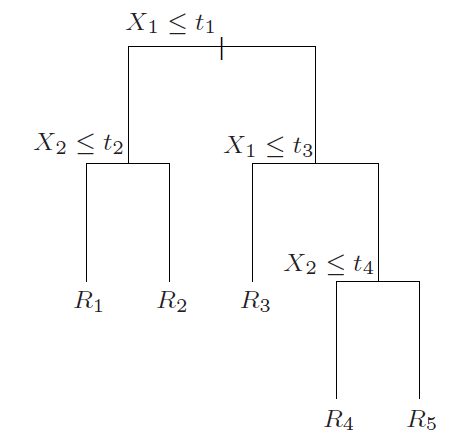
\includegraphics[width=.4\textwidth]{figure/regression_tree.png} %1.png是图片文件的相对路径
		\caption{回归决策树} %caption是图片的标题
		\label{img} %此处的label相当于一个图片的专属标志,目的是方便上下文的引用
	\end{figure}
	\item \textbf{[10pts]} 对于回归树,我们常采用平方误差来表示回归树对于训练数据的预测误差。但是找出平方误差最小化准则下的最优回归树在计算上一般是不可行的,通常我们采用贪心的算法计算切分变量$j$和分离点$s$。CART回归树在每一步求解如下优化问题
	$$\min _{j, s}\left[\min _{c_1} \sum_{x_{i} \in R_{1}(j, s)}\left(y_{i}-c_{1}\right)^{2}+\min _{c_{2}} \sum_{x_{i} \in R_{2}(j, s)}\left(y_{i}-c_{2}\right)^{2}\right]$$
	其中$R_1(j,s)=\{\boldsymbol{x}|x_j\leq s\},R_2(j,s)=\{\boldsymbol{x}|x_j>s\}$。试分析该优化问题表达的含义并给出变量$j,s$的求解思路。
\end{enumerate}
\begin{solution}\ \\
\begin{enumerate}[(1)]
	\item 将训练集同时当做评价指标,会使得划分时有可能过分考虑所选训练集内部特殊性的影响,将会导致过拟合
	\item 如图\\
	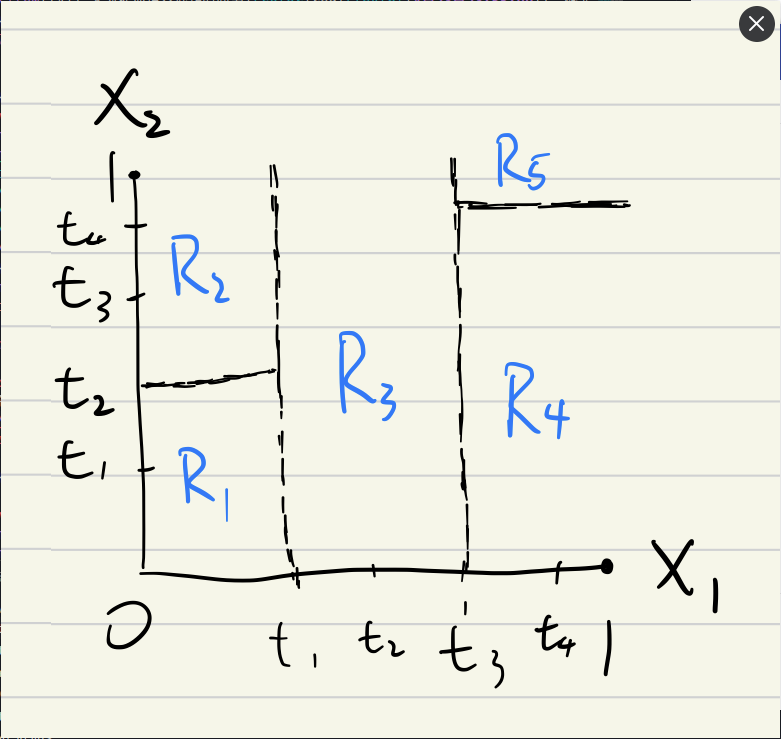
\includegraphics[width=0.8\textwidth]{figure/pr12.png}\\
	用线性模型来表示,使用4个分类器来对空间进行划分:
	$$\left\{
	\begin{aligned}
	&f(x_1,x_2)_{45,123} = x_1-t_3 \\
	&f(x_1,x_2)_{345,12} = x_1-t_1 \\
	&f(x_1,x_2)_{2,1} = x_2-t_2\\
	&f(x_1,x_2)_{5,4} = x_2-t_4
	\end{aligned}
	\right.
	$$
	*.参考机器学习导论课程群中助教对部分同学针对此题讨论的解答,这里给出另外一种依靠示性函数的线性模型分类方案\\
	\begin{equation*}
		\begin{split}
			f(X)=&\sum_{i=1}^5 i\mathbb{I}(X \in R_i)\\
			=&\mathbb{I}(X_1 \le t_1,X_2 \le t_2)+2\mathbb{I}(X_1 \le t_1, X_2 > t_2)\\
			&+3\mathbb{I}(t_1 < X_1 \le t_3)+4\mathbb{I}(X_1>t_3,X_2 \le X_4)\\
			&+5\mathbb{I}(X_1 > t_3, X_2 > t_4)\\
		\text{此时我们有}f(X) &= i \iff X \in R_i
		\end{split}
	\end{equation*}
	\item 表达的含义即求解在切分变量j和分离点s下,训练集上x关于变量j的“正类”、“负类”其对应y的类内方差之和最小的j,s。也就是寻找某个变量j和划分点s,使得这样划分后,两类的聚类程度最高。\\
			求解j,s的方法可以采用双重遍历,j自然是可以遍历的,s虽然是离散值,但是当其取值在$[x_k,x_{k+1}),x_1\le x_2 \le x_3...$时,他的作用是完全相同的,因此s可以离散化,于是就可以使用双重遍历找到最佳j与s的组合。
\end{enumerate}
\end{solution}

\section{[25pts] Decision Tree II}

\begin{enumerate}[(1)]
	\item \textbf{[5pts]} 对于不含冲突数据(即特征向量相同但标记不同)的训练集,必存在与训练集一致(即训练误差为$0$)的决策树。如果训练集可以包含无穷多个数据,是否一定存在与训练集一致的深度有限的决策树?证明你的结论。(仅考虑单个划分准则仅包含一次属性判断的决策树)
	\item \textbf{[5pts]} 考虑如表\ref{train data for tree}所示的人造数据,其中“性别”、“喜欢ML作业”是属性,“ML成绩高”是标签。请画出使用信息增益为划分准则的决策树算法所有可能的结果。(需说明详细计算过程)
	\begin{table}[h]
		\caption{训练集}
		\label{train data for tree}
		\centering
		\begin{tabular}{cccc}
			\hline 
			编号 & 性别 & 喜欢ML作业 & ML成绩高 \\ 
			\hline 
			1 & 男 & 是 & 是 \\ 
			2 & 女 & 是 & 是 \\ 
			3 & 男 & 否 & 否 \\ 
			4 & 男 & 否 & 否 \\ 
			5 & 女 & 否 & 是 \\ 
			\hline 
		\end{tabular}
	\end{table}
	\item \textbf{[10pts]} 考虑如表\ref{validation data for tree}所示的验证集,对上一小问的结果基于该验证集进行预剪枝、后剪枝,剪枝结果是什么?(需给出详细计算过程)
	\begin{table}[h]
		\caption{验证集}
		\label{validation data for tree}
		\centering
		\begin{tabular}{cccc}
			\hline 
			编号 & 性别 & 喜欢ML作业 & ML成绩高 \\ 
			\hline 
			6 & 男 & 是 & 是 \\ 
			7 & 女 & 是 & 否 \\ 
			8 & 男 & 否 & 否 \\ 
			9 & 女 & 否 & 否 \\ 
			\hline 
		\end{tabular}
	\end{table}
	\item \textbf{[5pts]} 比较预剪枝、后剪枝的结果,每种剪枝方法在训练集、验证集上的准确率分别为多少?哪种方法拟合能力较强?
\end{enumerate}

\begin{solution}\ \\
\begin{enumerate}[(1)]
	\item 假设数据属性值数量有限为n,因为不含冲突数据,所以即使有无穷多个数据,其中不重复的至多有$2^n$个。根据决策树的训练方法可知,每一个不重复的训练数据在完全展开的决策树上都对应到一个叶子节点,因此至多有$2^n$个叶子节点。对于有限叶子节点的树,其深度自然是有限的。但如果数据的属性值也是无限的,则无法产生有限深度决策树。
	\item 若不进行划分时ML成绩高占多数,因此单独一个节点为ML成绩高,此时信息熵\\
		  $Ent(D)=-(\frac{3}{5}lg\frac{3}{5}+\frac{2}{5}lg\frac{2}{5})=0.97$\\
		  此时若对性别进行划分,男:1,3,4:否,女:2,5:是,信息增益为\\
		  $Gain(D,sex)=Ent(D)-\frac{3}{5}(-\frac{1}{3}lg\frac{1}{3}-\frac{2}{3}lg\frac{2}{3})-\frac{2}{5}(-1lg1)=0.42$\\
		  此时若对喜欢ML作业进行划分,是:1,2:是,否:3,4,5:否,信息增益为\\
		  $Gain(D,love)=Ent(D)-\frac{2}{5}*0-\frac{3}{5}(-\frac{1}{3}lg\frac{1}{3}-\frac{2}{3}lg\frac{2}{3})=0.42$\\
		  两者信息增益相同,因此任意选择某一个作为第一划分属性,另一个作为下一个划分属性,所以共有如图两种决策树。\\
		  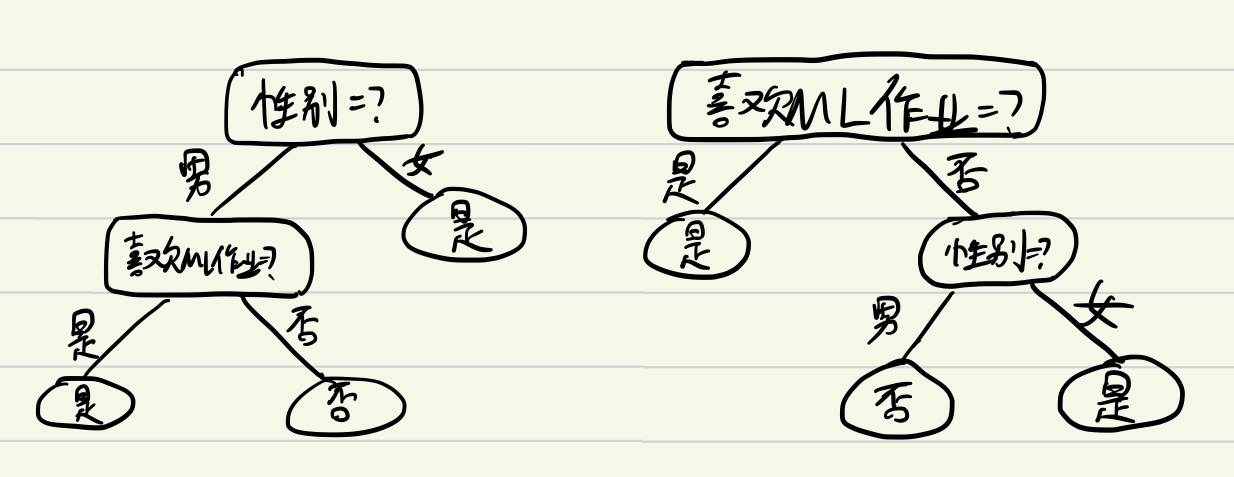
\includegraphics[width=0.95\textwidth]{figure/pr22.png}
	\item 左图,预剪枝:首先对于根节点,若不划分则“是”为多数,因此将所有判定为是,正确率$\frac{1}{4}$,若展开,则男“否”女“是”,正确率$\frac{1}{4}$,正确率不提高,因此不展开。
		  \\左图,后剪枝:对于最底部两个节点,若不剪枝则正确率为$\frac{1}{2}$,若剪枝则正确率为$\frac{1}{4}$,因此不剪枝。
		  \\右图,预剪枝:对根节点如果不展开,正确率$\frac{1}{4}$,展开正确率为$\frac{3}{4}$,因此此处展开。再看第二个划分点,若不划分则正确率$\frac{3}{4}$,若划分则正确率$\frac{1}{4}$,因此不展开。
		  \\右图,后剪枝:对底下两个节点,由上述分析可知剪枝导致正确率上升,因而剪枝,而根节点剪枝导致正确率下降,因而不剪枝。
		  \\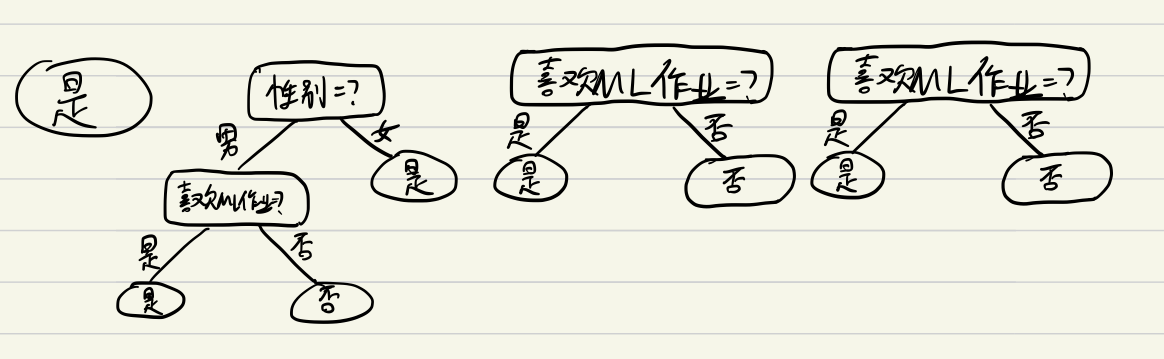
\includegraphics[width=0.95\textwidth]{figure/pr23.png}
	\item 对左图,预剪枝在训练集与测试集上准确率分别为$\frac{3}{5},\frac{1}{4}$,后剪枝为$1,\frac{1}{2}$
		  \\对右图,预剪枝后剪枝均为$\frac{4}{5},\frac{3}{4}$\\
		  经过对比可以发现后剪枝方法在训练集上拟合能力较强。
		\end{enumerate}
\end{solution}

\section{[25pts] SVM with Weighted Penalty}
考虑标准的SVM优化问题如下(即课本公式(6.35)),
\begin{equation}
\label{eq-svm}
\begin{split}
\min_{\mathbf{w},b,\xi_i}& \quad \frac{1}{2} \lVert \mathbf{w} \rVert^2 + C\sum_{i=1}^m\xi_i\\
\text{s.t.}&  \quad y_i(\mathbf{w}^\mathrm{T}\mathbf{x}_i + b)\geq 1-\xi_i\\
& \quad \xi_i \geq 0, i = 1,2,\cdots,m.
\end{split}
\end{equation}

注意到,在\eqref{eq-svm}中,对于正例和负例,其在目标函数中分类错误或分对但置信度较低的“惩罚”是相同的。在实际场景中,很多时候正例和负例分错或分对但置信度较低的“惩罚”往往是不同的,比如癌症诊断等。

现在,我们希望对负例分类错误(即false positive)或分对但置信度较低的样本施加$k>0$倍于正例中被分错的或者分对但置信度较低的样本的“惩罚”。对于此类场景下,

(1) \textbf{[10pts]} 请给出相应的SVM优化问题。

(2) \textbf{[15pts]} 请给出相应的对偶问题及KKT条件,要求详细的推导步骤。

\begin{solution}\ \\
\begin{enumerate}[(1)]
	\item 相应的SVM优化问题为:
	\begin{equation*}
	\begin{split}
	\min_{\mathbf{w},b,\xi_i}& \quad \frac{1}{2} \lVert \mathbf{w} \rVert^2 + C\sum_{i=1}^m k^{\frac{1-y_i}{2}} \xi_i\\
	\text{s.t.}&  \quad y_i(\mathbf{w}^\mathrm{T}\mathbf{x}_i + b)\geq 1-\xi_i\\
	& \quad \xi_i \geq 0, i = 1,2,\cdots,m.
	\end{split}
	\end{equation*}
	\item 对偶问题及KKT条件推导如下
	\begin{equation*}
	\begin{split}
		L(w,b,\xi,\alpha,\mu) &= \frac{1}{2} \lVert \mathbf{w} \rVert^2 + C\sum_{i=1}^m k^{\frac{1-y_i}{2}} \xi_i + \sum_{i=1}^m \alpha_i(1-\xi_i-y_i(w^T x_i+b)) - \sum_{i=1}^m \mu_i \xi_i \\
		&\text{其中}\alpha_i \ge 0,\mu_i \ge 0 \text{是拉格朗日乘子}\\
		&\text{令} L(w,b,\xi,\alpha,\mu) \text{对} w,b,\xi_i \text{偏导为零可得}\\
		w &= \sum_{i=1}^m\alpha_i y_i x_i\ \ \sum_{i=1}^m \alpha_i y_i = 0\ \ C k^{\frac{1-y_i}{2}} = \alpha_i + \mu_i\\
		&\text{将此三式带入可得}\\
		\theta(\alpha)&=\min_{w,b,\xi} L(w,b,\xi,\alpha,\mu)\\
		&=\frac{1}{2}\lVert \sum_{i=1}^m \alpha_i y_i x_i \rVert + \sum_{i=1}^m \alpha_i - \sum_{i=1}^m \alpha_i y_i (\sum_{i=1}^m \alpha_i y_i x_i)^T x_i\\
		&=\sum_{i=1}^m \alpha_i-\frac{1}{2}\lVert \sum_{i=1}^m \alpha_i y_i x_i \rVert\\
		&=\sum_{i=1}^m \alpha_i-\frac{1}{2}\sum_{i=1}^m \sum_{j=1}^m \alpha_i \alpha_j y_i y_j x_i^T x_j\\
		&\text{所以对偶问题为}\\
		\max_{\alpha} \quad &\sum_{i=1}^m \alpha_i-\frac{1}{2}\sum_{i=1}^m \sum_{j=1}^m \alpha_i \alpha_j y_i y_j x_i^T x_j\\
		\text{s.t.} \quad &\sum_{i=1}^m\alpha_i y_i = 0,\\
		&0 \le \alpha_i \le C k^{\frac{1-y_i}{2}}, \quad i=1,2,\dots,m.\\
		&\text{KKT条件为}\\
		&\left\{
		\begin{aligned}
		&w= \sum_{i=1}^m\alpha_i y_i x_i\ \ \sum_{i=1}^m \alpha_i y_i = 0\ \ C k^{\frac{1-y_i}{2}} = \alpha_i + \mu_i \\
		&y_i(\mathbf{w}^\mathrm{T}\mathbf{x}_i + b)+\xi_i -1 \ge 0 \quad \xi_i \geq 0\\
		&\alpha \ge 0 \quad \mu_i \ge 0\\
		&\alpha_i(y_i(\mathbf{w}^\mathrm{T}\mathbf{x}_i + b)+\xi_i -1) = 0 \quad \mu_i \xi_i = 0
		\end{aligned}
		\right.
	\end{split}
	\end{equation*}
\end{enumerate}
\end{solution}

\section{[30 pts] 编程题, Linear SVM}
\textbf{请结合编程题指南进行理解}

SVM转化成的对偶问题实际是一个二次规划问题,除了SMO算法外,传统二次规划方法也可以用于求解对偶问题。求得最优拉格朗日乘子后,超平面参数$\mathbf{w,b}$可由以下式子得到:
\begin{equation}
\mathbf{w} = \sum_{i=1}^m \alpha_i y_i x_i
\end{equation}
\begin{equation}
\mathbf{b} = \frac{1}{|S|}\sum_{s\in S} (y_s-\sum_{i\in S}\alpha_i y_i x_i^T x_s)
\end{equation}
请完成以下任务:
\begin{enumerate}[(1)]
	\item \textbf{[5pts]} 使用QP方法求解训练集上的SVM分类对偶问题(不考虑软间隔情况)。
	\item \textbf{[10 pts]} 手动实现SMO算法求解上述对偶问题。
	\item \textbf{[15 pts]} 对测试数据进行预测,确保预测结果尽可能准确。
\end{enumerate}

\begin{solution}\ \\
	\begin{enumerate}[(1)]
		\item 对偶问题为
		\begin{equation*}
		\begin{split}
			\max_\alpha \quad &\sum_{i=1}^m\alpha_i -\frac{1}{2}\sum_{i=1}^m\sum_{j=1}^m\alpha_i\alpha_jy_iy_jx_i^Tx_j\\
			s.t. \quad &\sum_{i=1}^m \alpha_i y_i = 0,\\
			&\alpha_i \ge 0,\quad i=1,2,\dots,m.
		\end{split}
		\end{equation*}
		将其化为标准二次规划问题为
		\begin{equation*}
		\begin{split}
			\min_\alpha \quad &\frac{1}{2}\alpha^T P \alpha + q^T \alpha\\
			s.t. \quad &G\alpha \preceq h\\
			&A\alpha = b
		\end{split}
		\end{equation*}
		其中
		\begin{equation*}
		\begin{split}
			P_{ij} &= y_iy_jx_i^Tx_j\\
			q_i &= -1,\ i=1,2,\dots,m\\
			G &= -I\\
			h &= 0,\ i=1,2,\dots,m\\
			A_{i} &= y_i, \ i=1,2,\dots,m\\
			b &= 0
		\end{split}
		\end{equation*}
		使用cvxopt包进行求解即得答案

		\item 参考课本内容以及https://zhuanlan.zhihu.com/p/29212107上对于SMO算法的讲解,手动实现了SMO算法优化上述对偶问题,并根据w,b的表达式进行最终模型生成
		\item 针对前两问的数据,将xtrain拆分出一部分为xvalid,以对训练的模型进行评估,并选取正确率较高的方法作为最终预测ytest的评估
	\end{enumerate}
\end{solution}

\end{document}